\section{Application: Wait Time at Canadian Airports}
By providing efficient and effective \textbf{pre-board screening} (PBS), the \textit{Canadian Air Transport Security Authority} (CATSA) ensures the safety of all passengers and crew aboard flights departing Canadian airports while maintaining an appropriate balance between staffing and the wait time experienced by passengers. \par The number of active screening stations and the number of passengers affect the wait times, and, as a result, budget cuts have a strong impact on the system, both in Canada and in the United States.\newl
Numerous factors influence the wait time at PBS checkpoints at Canadian airports: the schedule intensity of departing flights, the volume of passengers on these flights, the number of servers and processing rates at a given checkpoint, etc. \par One of CATSA's goals is to ensure that the pre-board screening experience at Canadian airports is made as efficient as possible by minimizing the waiting time at checkpoints. With this in mind, the \textbf{Wait-Time Impact Model} (WTIM) was designed to achieve the following tasks: 
\begin{enumerate}[noitemsep]
\item provide estimates of the passenger arrival rates $\lambda$, the processing rates $\mu$ and the number of servers $c$ at each checkpoints, using available field data;
\item calculate the Quality of Service (QoS) level $(p_x,x)$  and determine what service level can be achieved at each checkpoint (i.e. the percentage $p$ of passengers which will wait less than $x$ minutes, for $x$ fixed) for a given arrival rate $\lambda$, processing rate $\mu$, number of servers $c$;
\item provide the average number of servers $c^*$ required to achieve a prescribed QoS level $(p_x,x)$, given an arrival profile $\lambda^*$;
\item provide quality of service (QoS) level curves $(p_x (x),x)$ (i.e. cumulative distribution curves) under various arrival rate and number of active servers for each checkpoint (where $x$ is allowed to vary).\end{enumerate}
The \begin{figure*}[!t]
\centering
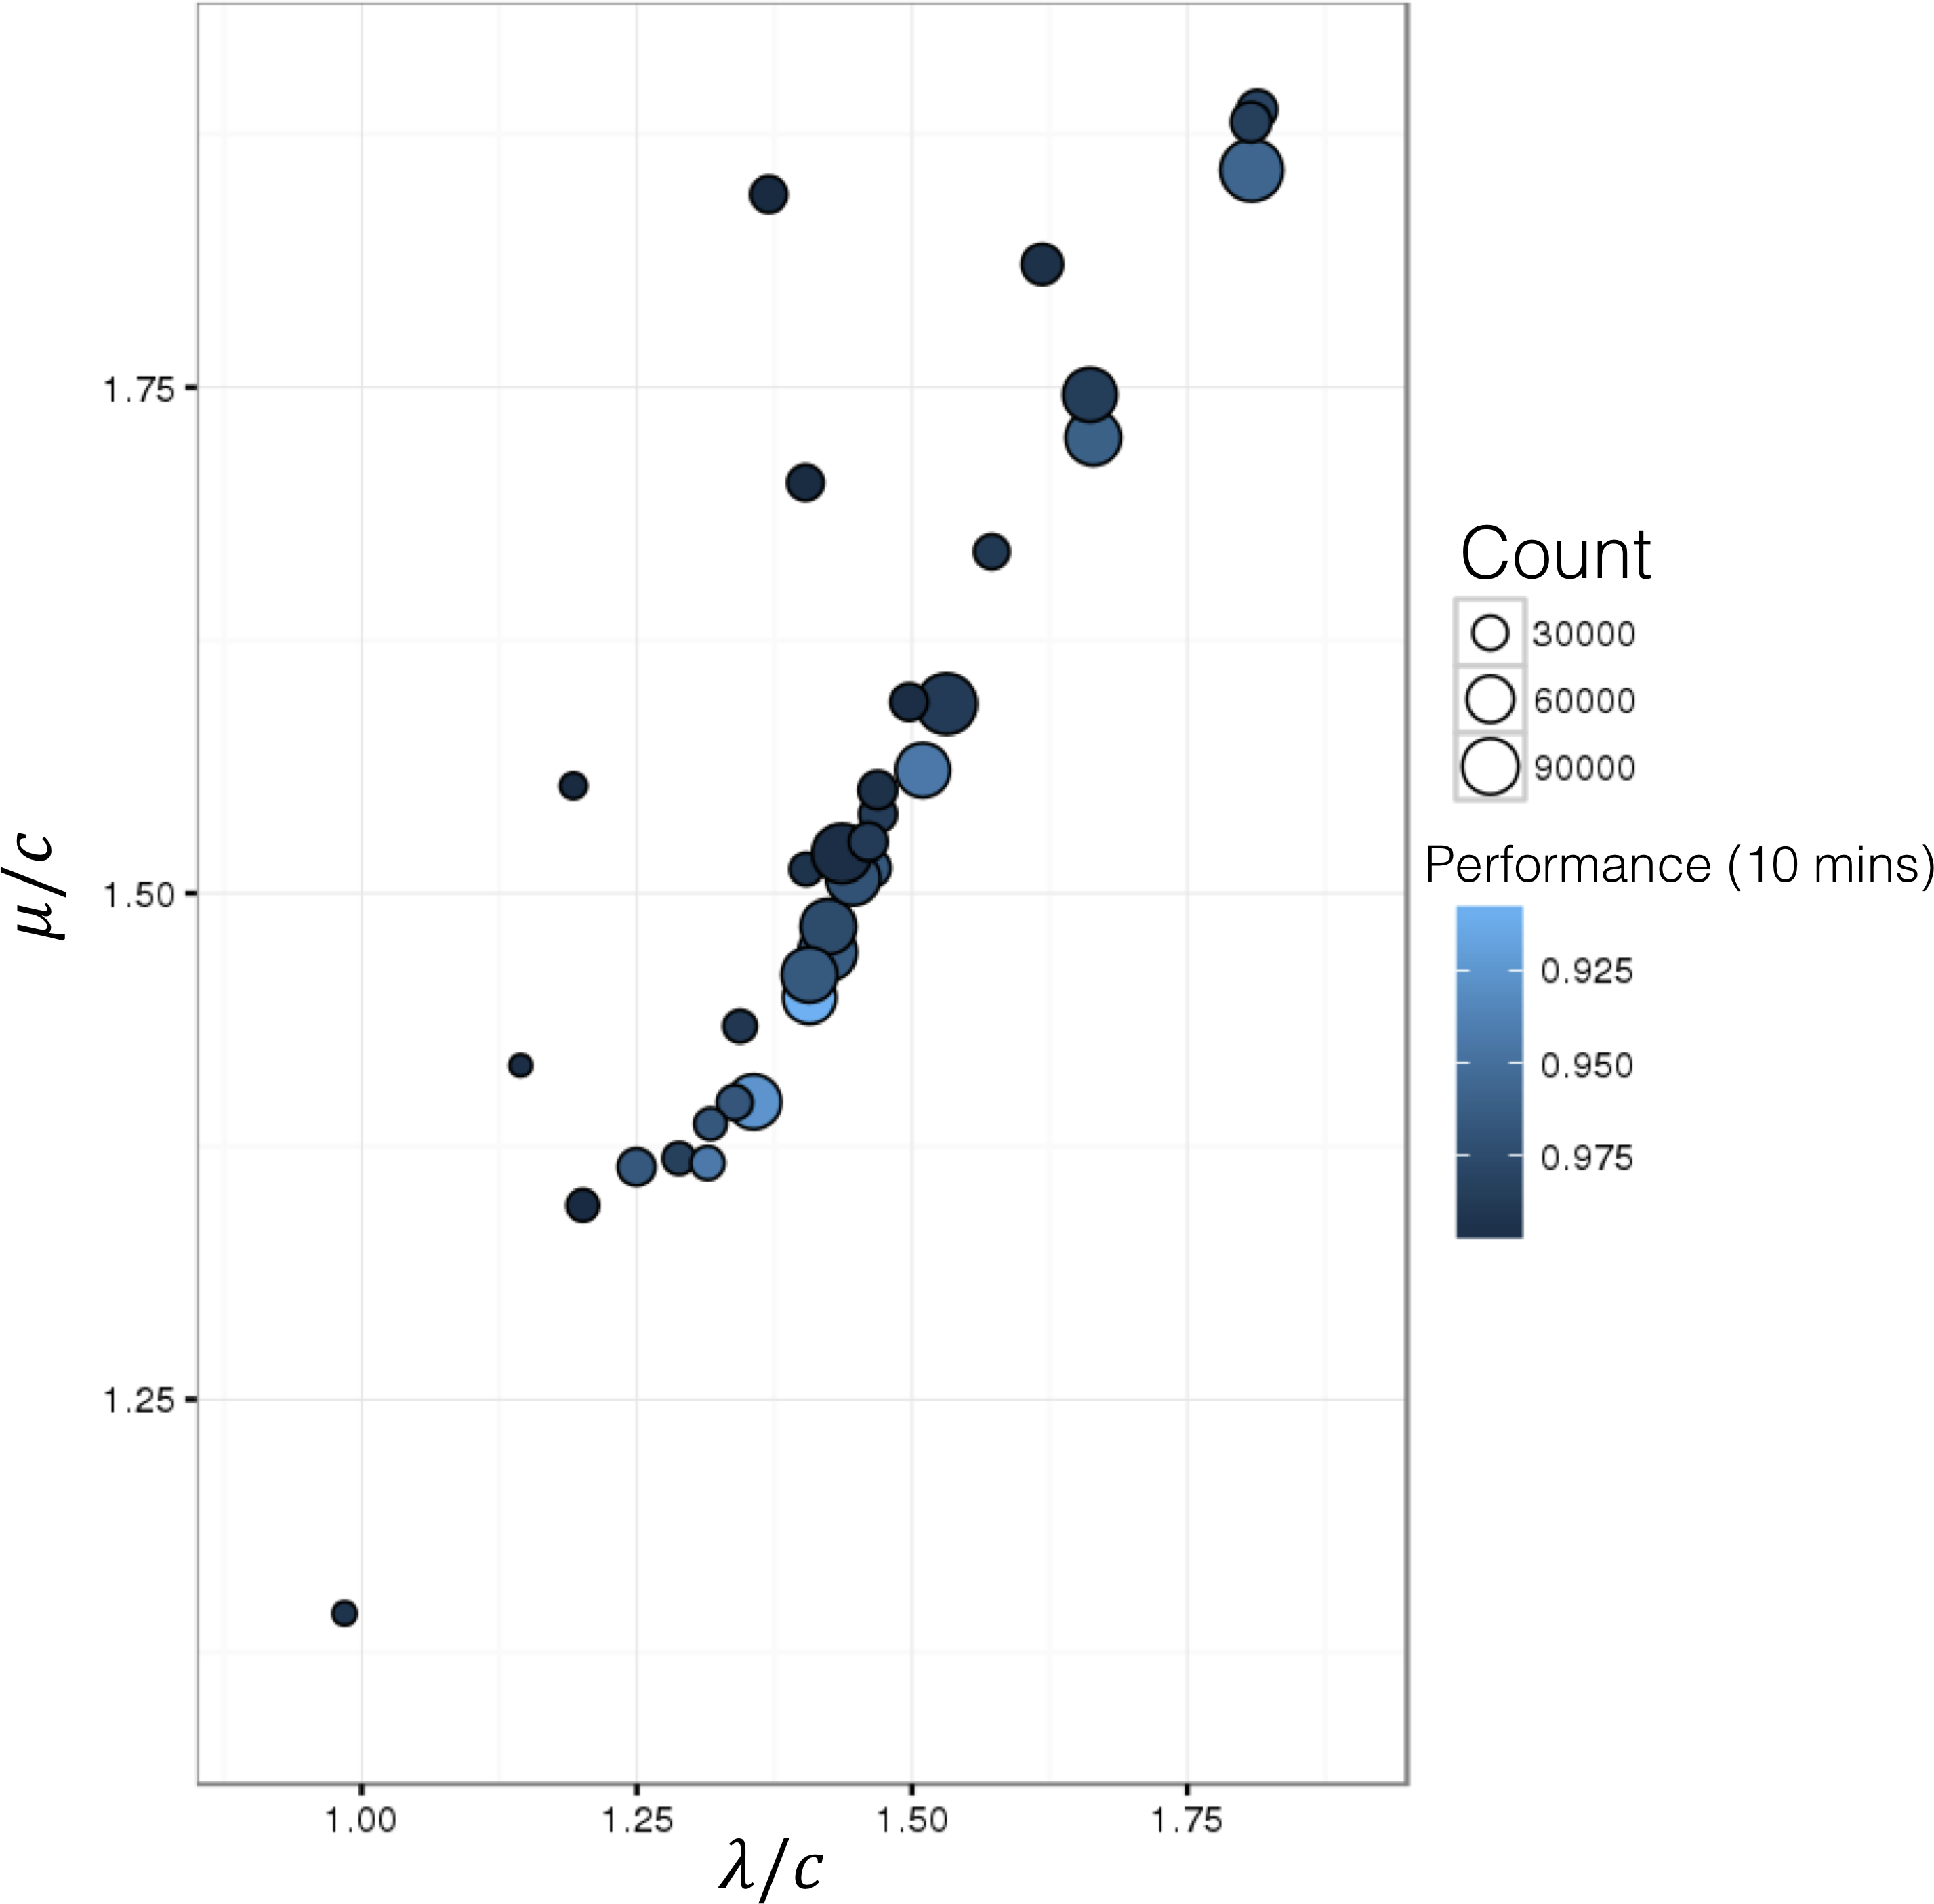
\includegraphics[height=0.43\textheight]{Images/CATSA2.png}\quad 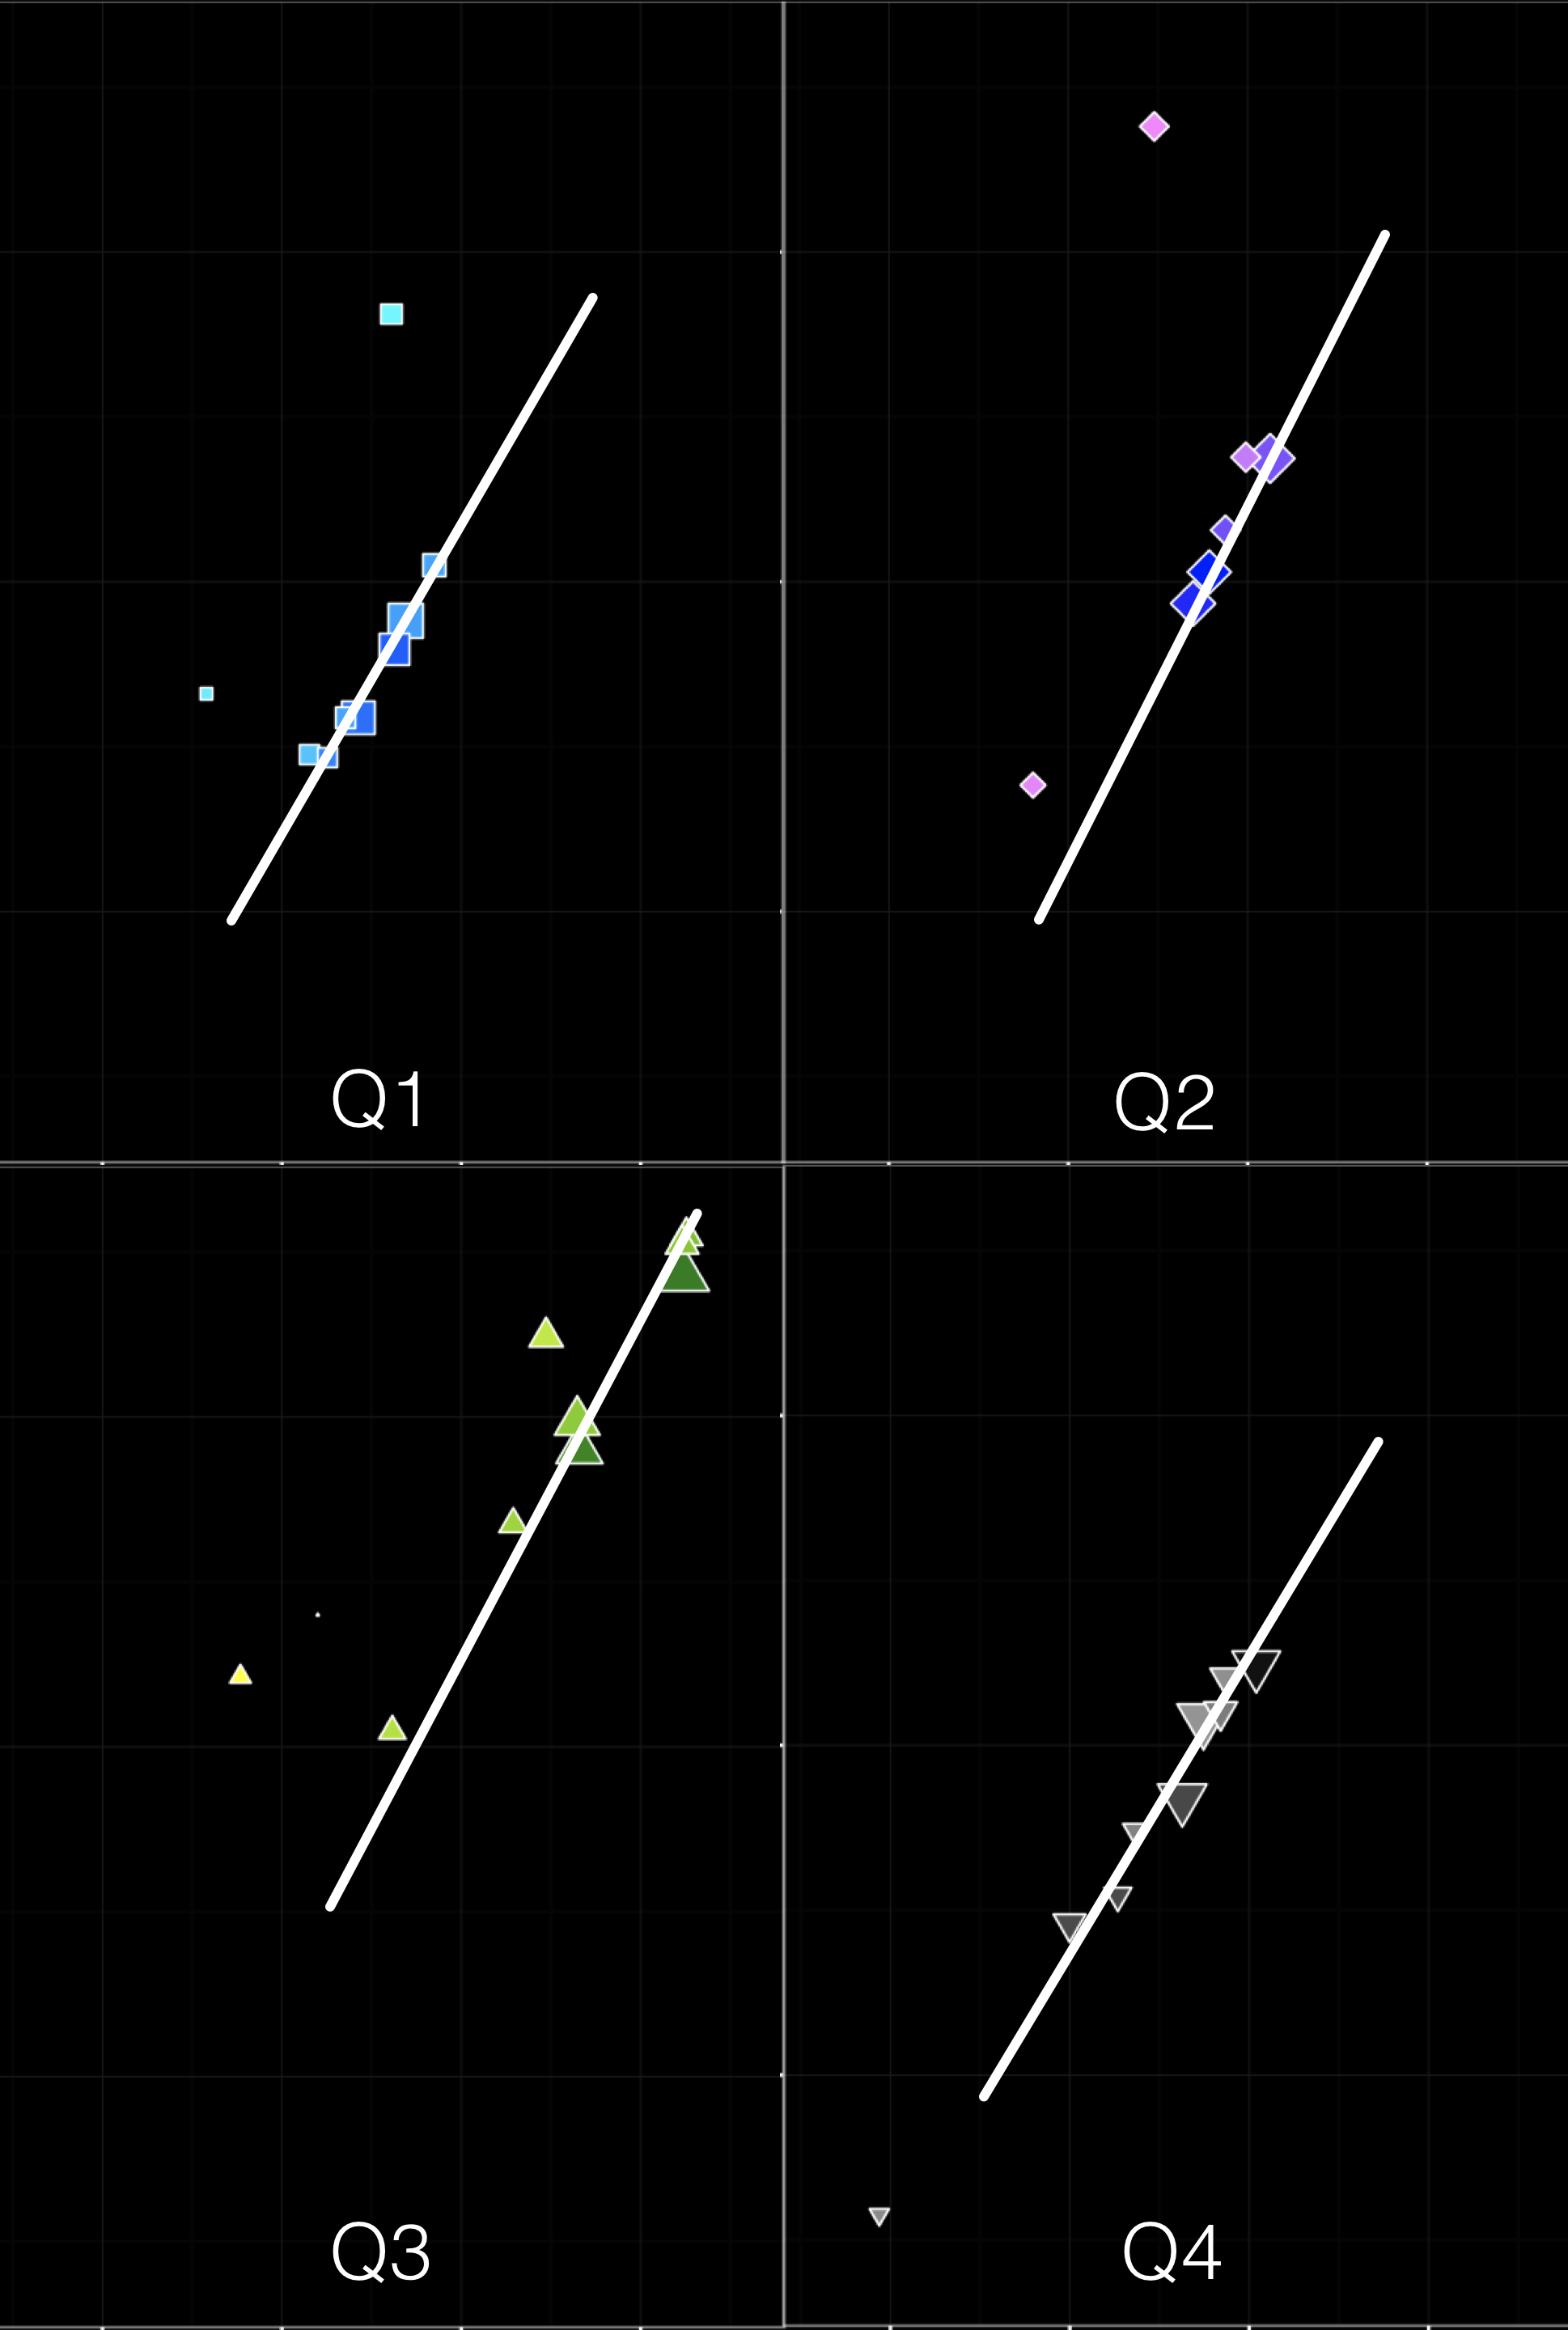
\includegraphics[height=0.43\textheight]{Images/CATSA3.png} \\  \ \\ 
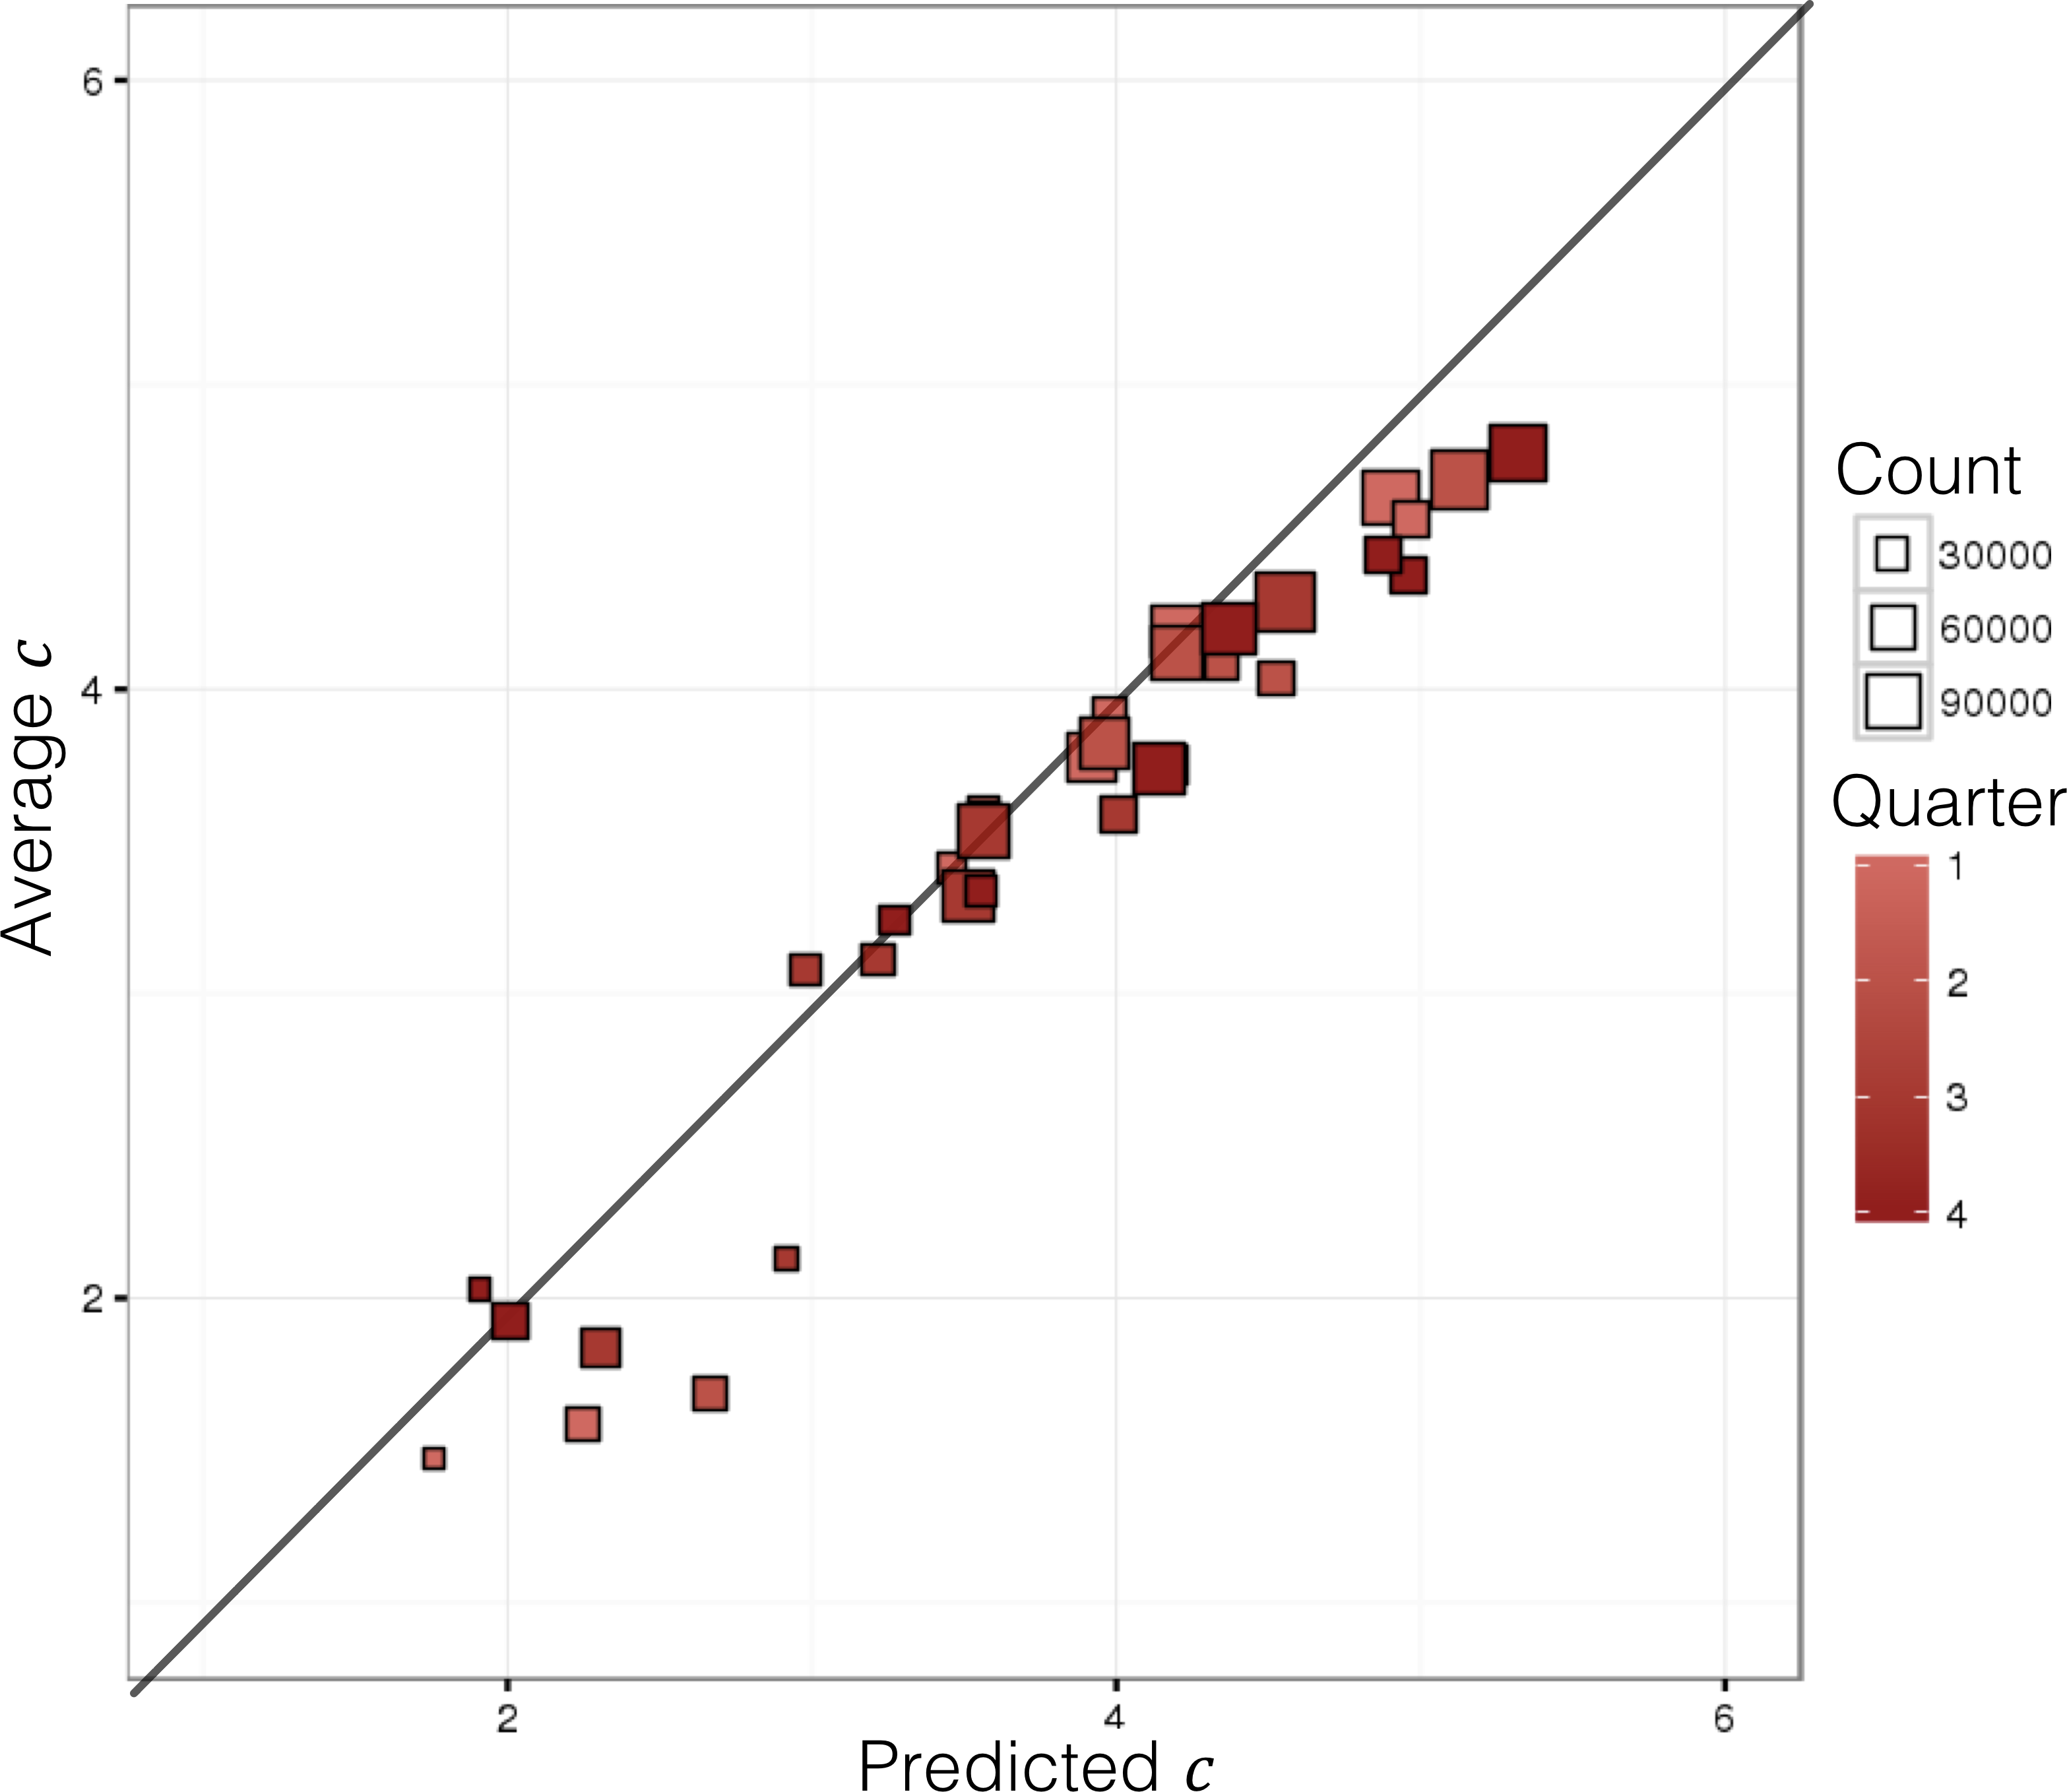
\includegraphics[width=0.65\textwidth]{Images/CATSA4.png}  
\caption{\small Top row: visualisation of a specific checkpoint's queueing parameters -- $\lambda$, $\mu$, $\bar{c}$, passenger count, and performance (percentage of travellers waiting less than 15 minutes to be screened); the relationship between $\lambda/\bar{c}$ and $\mu/\bar{c}$ is practically linear (left), which is easier to see at the quarter level (right). Bottom row: Predicted average number of server against actual number of server required to maintain prescribed performance, with passenger count, by quarter. The perfect prediction line is added for ease of comparison.}\label{fig:checkpoint}
\end{figure*} queueing structure leads to some interesting insights  (see Figure~\ref{fig:checkpoint}). More details are available in the accompanying presentation. 